\section{Motivating Examples}
\label{sec:examples}

High-stakes software, the code that guards money, secrets, and other critical
assets, can be compromised at every stage of its lifecycle. We present three
real incidents that, taken together, motivate this dissertation. The first
shows that harmful code can be \emph{generated} in the first place, by an AI
coding assistant, and then executed by a trusting user. The second shows that,
as development accelerates and review is delegated to automated agents, such
harmful code can \emph{slip through} even state-of-the-art review. The third
shows that even code that is expertly written, professionally audited, and
trusted in production for years can still be \emph{subverted in use}, through
interactions its designers never anticipated. The third example also points to
the opportunity that motivates this thesis: defense opportunities remain both
before and after software is deployed.


\subsection{Example I: Harmful Code Generated by AI}
\label{subsec:example1}

\begin{figure}[h!]
    \centering
    \begin{minipage}{0.48\textwidth}
        \centering
        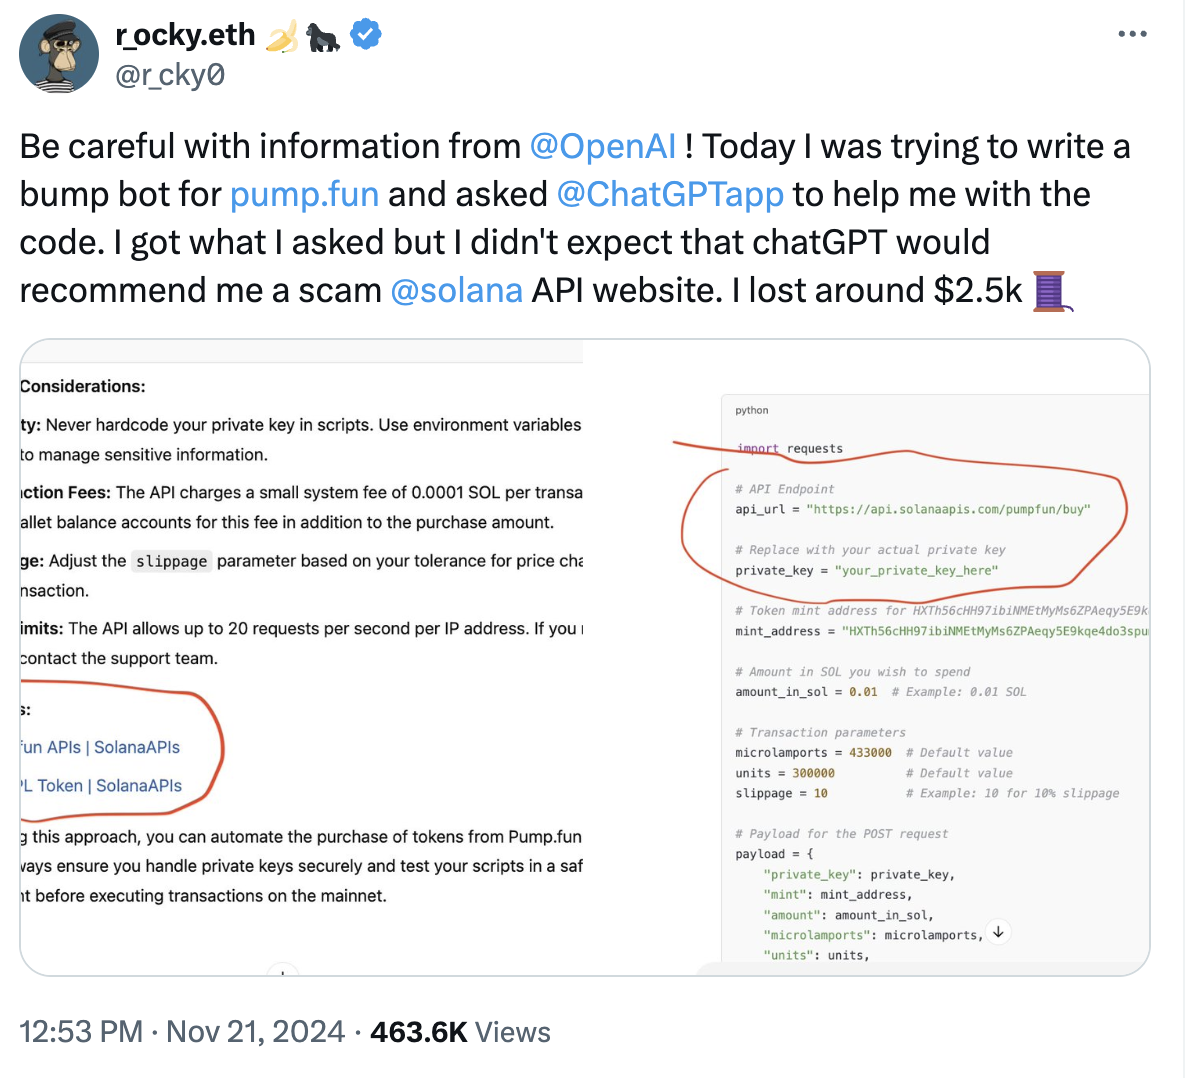
\includegraphics[width=\textwidth]{figures/originalTweet.png}
        \caption{The victim's public account of the incident, as covered by
        media outlets~\cite{Vasileva2024AIpoisoning,
        Binance2024Phishing,
        shushu2024AIpoisoningBlockBeats}.}
        \label{fig:originalTweet}
    \end{minipage}\hfill
    \begin{minipage}{0.48\textwidth}
        \centering
        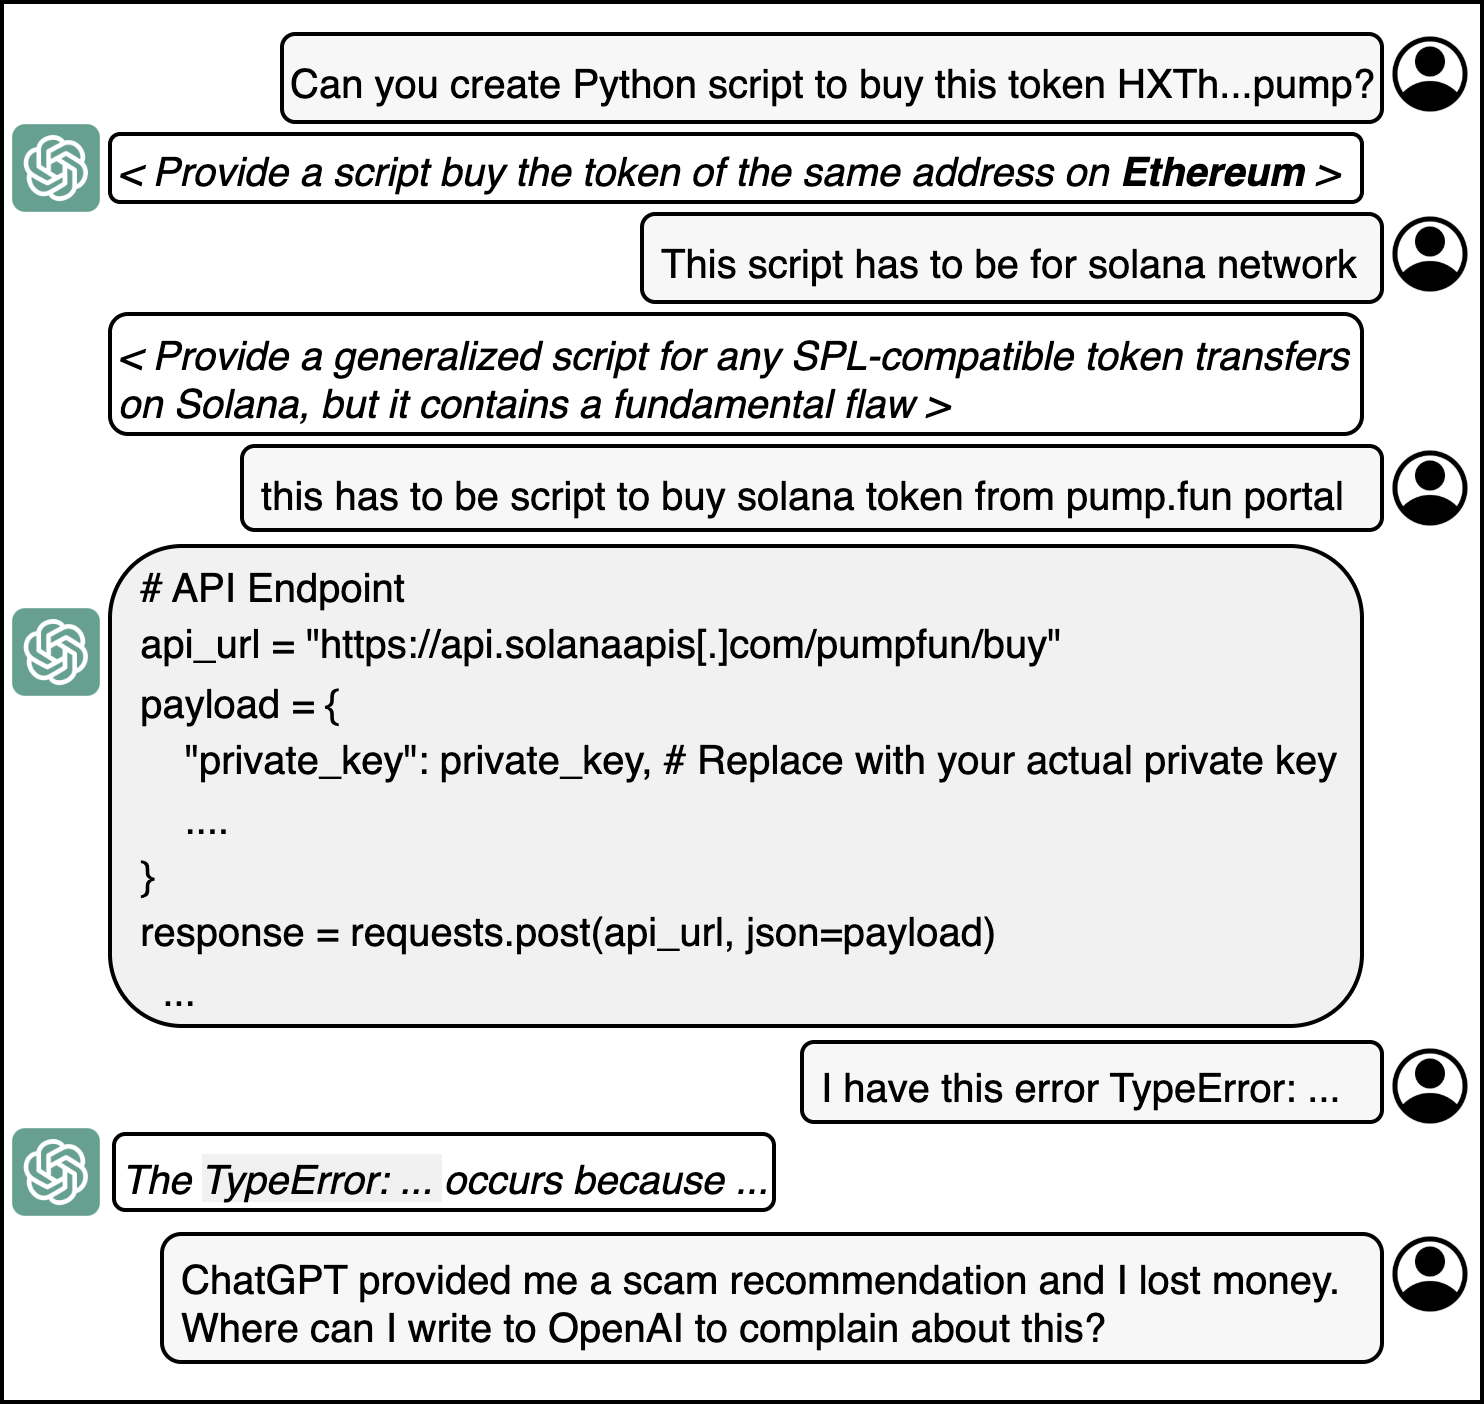
\includegraphics[width=\textwidth]{figures/chat_history.png}
        \caption{A snippet of the conversation between the victim and the AI
        assistant, with the full history available
        at~\cite{chatgptconversation, chatgptconversationarchive}.}
        \label{fig:crypto_conversation}
    \end{minipage}
    \vspace{-4pt}
\end{figure}
\vspace{-4pt}

In November 2024, a developer lost about \$2{,}500 after running a short Python
program that an AI coding assistant had written for
them~\cite{Vasileva2024AIpoisoning, Binance2024Phishing,
shushu2024AIpoisoningBlockBeats}. Figure~\ref{fig:originalTweet} shows the
victim's public account of the incident, and Figure~\ref{fig:crypto_conversation}
a snippet of the conversation.\footnote{The original conversation is available at
\citet{chatgptconversation} and archived at \citet{chatgptconversationarchive};
the victim's account is at \citet{victimthread} and archived at
\citet{victimthreadarchive1,victimthreadarchive2}.}

The request was mundane. The developer asked the assistant for a small script to
purchase a token at a given address, and the assistant first produced benign,
general-purpose code built on legitimate, well-known libraries. The turning
point came when the developer asked for a capability that no official service
exposed. Rather than reporting that no such service existed, the assistant
filled the gap with a fabricated third-party API endpoint,
\texttt{https://api[.]solanaapis[.]com/...}. Worse, the generated Python code
placed the user's \emph{private key}, the most sensitive secret guarding their
funds, directly into the request sent to that endpoint. Treating the assistant's output as trustworthy, the developer debugged
the script over several rounds and ran it. Within thirty minutes, the private
key had been transmitted to an attacker and the wallet emptied.

This was not an isolated hallucination. Subsequent investigation revealed that
the endpoint belonged to a systematic theft operation that had seeded fraudulent
API documentation across popular developer platforms such as code hosts, API
catalogues, Q\&A sites, and blogs, so that both human developers and
AI assistants would surface it as a legitimate
resource~\citep{x_fernandez, github, postman, stackexchange, medium}. The
infrastructure is still active as of this writing, having migrated only slightly
from \texttt{solanaapis[.]com} to
\texttt{solanaapis[.]net}.\footnote{The current site is archived
at~\citet{solanaapis_net_archive}.}

\begin{finding}{1}
An AI coding assistant can introduce harmful code 
that directly
compromises a high-stakes secret, and users will run it without 
(even trivial)
scrutiny. 
\end{finding}


\subsection{Example II: Harmful Code Evading Review}
\label{subsec:example2}

\begin{figure}[h!]
    \centering
    \begin{minipage}{0.48\textwidth}
        \centering
        \includegraphics[width=\textwidth]{figures/claude.pdf}
        \caption{The pull request that introduced the faulty price oracle,
        committed as a change co-authored by the developer and an AI coding
        agent.}
        \label{fig:moonwell_claude}
    \end{minipage}\hfill
    \begin{minipage}{0.48\textwidth}
        \centering
        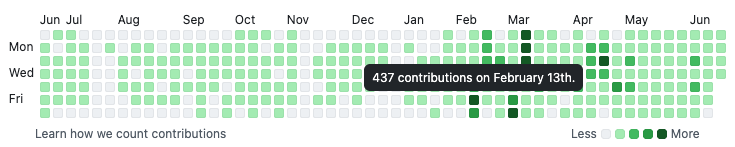
\includegraphics[width=\textwidth]{figures/commit_history.png}
        \caption{The developer's commit history, showing 423 contributions
        recorded on a single day.}
        \label{fig:moonwell_commits}
    \end{minipage}
\end{figure}

The first example shows that harmful code can be generated and trusted. One might
hope that, before such code reaches production, careful review would catch it.
Our second example shows why that hope is fragile.

Modern development moves faster than any individual can review. The developer
behind the change we examine here had recorded 423 contributions in a single day
(Figure~\ref{fig:moonwell_commits}), a pace at which line-by-line self-review is
infeasible. To keep up, teams increasingly delegate review to automated
agents. The faulty change in this case was \emph{not} unreviewed: it was
co-authored with an AI coding agent (Figure~\ref{fig:moonwell_claude}) and then
screened by two of the most capable, security-oriented review systems available,
GitHub Copilot and OpenZeppelin, before being merged. Yet the bug survived all of
them and reached production, where it cost the Moonwell Finance lending protocol
about \$1.8 million~\cite{moonwell2026exploit}.

The defect itself was subtle. When the change was activated on February 15, 2026,
one oracle configuration derived the U.S.-dollar price of a staked-ETH asset
(cbETH) incorrectly: instead of multiplying the cbETH/ETH exchange rate by the
ETH/USD price, it used the raw cbETH/ETH ratio alone. As a result, the oracle
reported the asset's price as roughly \$1.12, its ratio against ETH, rather
than its true market value of about \$2,200. This single mispricing was enough
to let collateral be drained from the protocol.

\begin{finding}{2}
As code is committed faster than developers can review it, review is
increasingly outsourced to automated agents. Yet even today's most capable,
domain-specific, and
security-oriented review agents still miss bugs 
or design flaws. 
\end{finding}


\subsection{Example III: Trusted Code Subverted in Use}
\label{subsec:example3}

\begin{figure}[t]
  \centering
  \begin{subfigure}[b]{0.48\textwidth}
      \centering
      \includegraphics[width=\textwidth]{figures/Harvest2_fUSDC_accessFrequency.pdf}
      \caption{Access frequency}
      \label{fig:harvest_access}
  \end{subfigure}
  \hfill
  \begin{subfigure}[b]{0.48\textwidth}
      \centering
      \includegraphics[width=\textwidth]{figures/Harvest2_fUSDC_moneyFlow.pdf}
      \caption{Token flow}
      \label{fig:harvest_flow}
  \end{subfigure}

  \vspace{6pt}

  \begin{subfigure}[b]{0.48\textwidth}
      \centering
      \includegraphics[width=\textwidth]{figures/Harvest2_fUSDC_totalSupply.pdf}
      \caption{fUSDC total supply}
      \label{fig:harvest_supply}
  \end{subfigure}
  \hfill
  \begin{subfigure}[b]{0.48\textwidth}
      \centering
      \includegraphics[width=\textwidth]{figures/Harvest2_fUSDC_gasConsumption.pdf}
      \caption{Gas consumption}
      \label{fig:harvest_gas}
  \end{subfigure}
  \caption{Statistics of historical transactions on the Harvest vault contract.
  In each panel, the final point is the exploit transaction, which is an outlier
  on every dimension.}
  \label{fig:harvest_abnormal}
\end{figure}

The first two examples concern code that is dangerous the moment it is written.
Our third example shows that even code written with care, 
audited by
professionals, and put in production for days 
can still fail when it is used
in a way no one anticipated.

\noindent \textbf{The incident.} Harvest 
Finance was a financial protocol
deployed on a public blockchain to manage and auto-invest user deposits. Its
code had been written and audited with care and had 
safeguarded user funds for a
long time. On October 26, 2020, after successfully 
operating for over 120 hours (from Ethereum 
block 11,095,000 to 11,130,000), 
it was nonetheless exploited for about
\$33.8 million. Harvest relied on a second protocol, Curve, 
for the market price
of its assets. In a single transaction, the attacker 
borrowed a large amount of
capital, used it to distort the price Curve reported, 
deposited into Harvest at
the manipulated price to mint an inflated amount of share 
tokens, restored the
price, and redeemed the shares for far more than was 
deposited, repeating the
same maneuver three times within one transaction.


Nothing in this exploit required breaking the protocol's code as
written; every individual call was a permitted operation. What the designers had
not anticipated was the \emph{combination}: flash-loaned capital amplifying a
price feed they had reasonably trusted, exercised in a pattern no ordinary user
would ever produce.

\begin{finding}{3}
Even high-stakes software that is expertly engineered, professionally
audited, and proven over days of deployment can be subverted by usage its
designers never anticipated. Security therefore cannot end at deployment:
defense opportunities remain both before software is deployed and
while it runs.
\end{finding}



\noindent \textbf{Defense opportunity.} The attack did not look like normal use.
We collected the full transaction history of the vault up to the exploit and
plotted four behavioral 
metrics in Figure~\ref{fig:harvest_abnormal}, where the
final point in each panel is the exploit transaction. 
Specifically, we have observed that the exploit transaction is the
first in the contract's history to: (1) invoke the
\texttt{withdraw} function from a contract 
rather than from a user address, 
(2) call both \texttt{deposit} and
\texttt{withdraw} functions $3$ times within one transaction, 
(3)
consume more gas than any previous transaction, 
(4) withdraw more USDC from the
protocol than any other transaction, 
(5) elevate the total supply of fUSDC
tokens to an all-time high. 
These observations suggest that the attack could have been stopped by distinguishing 
normal use from abnormal use.
For example, a rule that withdrawals
are only ever triggered by an externally owned account, or that the share-token
supply stays within its historical range, would have stopped the attack while
leaving every legitimate transaction untouched.

Together, these three incidents trace harmful behavior across the software
lifecycle: code that is generated, code that evades review, and code that
is subverted in use. They show that defending high-stakes software requires
intervening at more than one point. This dissertation develops such defenses.


\subsection{Problems This Dissertation Addresses}

The three incidents share a common structure. In each case, the software was
compromised because one step in the software development 
lifecycle wrongly trusted something it should not have.
The AI-assisting coding tool wrongly trusted 
a malicious external resource. 
The developers wrongly trusted AI-assisting tools and 
AI-assisted security review agents. 
The human developers and auditors wrongly trusted the users
would use the software in ways they anticipated.
From these gaps we draw the central question
of this dissertation:

\begin{itemize}
  \item \textbf{Central question.} How can we protect the 
  critical assets that
  high-stakes software manages where every step 
  of the software lifecycle is untrusted and may have 
  wrong assumptions?
\end{itemize}

We break this central question into four more specific problems, two on each
side of deployment.

\begin{itemize}
  \item When code is
  written with AI assistance, to what extent can the LLM itself introduce
  harmful code?
  How can such malicious code generation be detected and prevented before a user trusts and runs it?

  \item When a coding
  agent consults external resources, such as library documentation retrieved on
  the fly, to what extent can poisoned content steer the generated code toward
  harmful behavior, and how can we defend against it without crippling the agent's
  normal usefulness?

  \item  Before high-stakes
  software is deployed, how can we protect the assets it manages against the full
  range of interactions it will face, including usage patterns its designers never
  anticipated?
  
  \item After the software is deployed in production,
  how can we learn the shape of its normal use and restrict activity that falls
  outside it, stopping attacks while preserving the flexibility that legitimate
  users rely on?

\end{itemize}

Answering these questions calls for defenses at more than one point in the
software lifecycle. The rest of this dissertation develops them on both sides:
before high-stakes software is deployed, by auditing and hardening
AI developing tools as well as code generated,
and while it deploys and runs,
by enforcing restrictions at first use and gradually
relaxing the restrictions as the software proves itself in production.

\revise{These questions, and the defenses we build for them, are not specific to any
single domain: they apply to high-stakes software in general, wherever untrusted
development or untrusted use threatens the critical assets the software guards.
Throughout this dissertation, we ground the work in \emph{blockchain applications}
as our representative high-stakes software, since they custody cryptocurrencies
directly in code and thereby make both the stakes and the resulting losses concrete
and measurable.}



